\section{案例研究:对 RC4 流密码的密码学分析}\label{sec:3-9}

RC4 流密码由 Ron Rivest 在 1987 年设计,历史上曾用于(在 SSL/TLS 协议中)保护网络流量和(在 802.11b WEP 协议中)保护无线流量的安全。它被设计成可在内存很小的 $8$ 位处理器上运行。虽然 RC4 仍在使用,但它已被证明容易遭受一些显著的攻击,因而不应该被应用在新的项目中。我们对 RC4 的讨论可以作为流密码分析的一个优雅的例子。

RC4 密码的核心是一个 PRG,称为 RC4 PRG。该 PRG 维护一组内部状态,包含一个 $256$ 字节的数组 $S$ 和两个额外的字节 $i,j$,作为指入 $S$ 的两个指针。数组 $S$ 包含 $\{0,\dots,255\}$ 中的所有的数字,且每个数字正好出现一次。图 \ref{fig:3-12} 给出了一个 RC4 状态的例子。

\begin{figure}
	\centering
	

\tikzset{every picture/.style={line width=0.9pt}} %set default line width to 0.75pt        

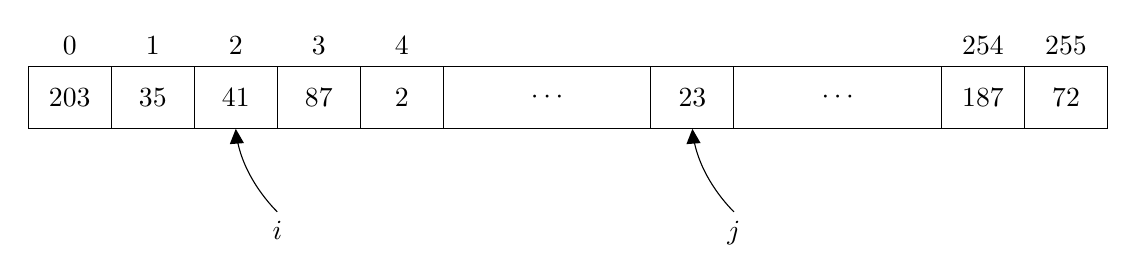
\begin{tikzpicture}[x=0.75pt,y=0.75pt,yscale=-1,xscale=1]
%uncomment if require: \path (0,125); %set diagram left start at 0, and has height of 125

%Shape: Rectangle [id:dp8774291212656176] 
\draw   (0,20) -- (520,20) -- (520,50) -- (0,50) -- cycle ;
%Straight Lines [id:da7417447618175568] 
\draw    (40,20) -- (40,50) ;
%Straight Lines [id:da7781155181250581] 
\draw    (80,20) -- (80,50) ;
%Straight Lines [id:da46532313693800553] 
\draw    (120,20) -- (120,50) ;
%Straight Lines [id:da891858566523396] 
\draw    (160,20) -- (160,50) ;
%Straight Lines [id:da9416263498656987] 
\draw    (200,20) -- (200,50) ;
%Straight Lines [id:da9145178928639244] 
\draw    (300,20) -- (300,50) ;
%Straight Lines [id:da9586008500216805] 
\draw    (340,20) -- (340,50) ;
%Straight Lines [id:da14035841668976134] 
\draw    (440,20) -- (440,50) ;
%Straight Lines [id:da2555764265900269] 
\draw    (480,20) -- (480,50) ;
%Curve Lines [id:da39731890421371974] 
\draw    (120,90) .. controls (112.82,82.82) and (102.51,69.12) .. (100.3,52.86) ;
\draw [shift={(100,50)}, rotate = 85.75] [fill={rgb, 255:red, 0; green, 0; blue, 0 }  ][line width=0.08]  [draw opacity=0] (7.14,-3.43) -- (0,0) -- (7.14,3.43) -- cycle    ;
%Curve Lines [id:da10312523213104918] 
\draw    (340,90) .. controls (332.82,82.82) and (322.51,69.12) .. (320.3,52.86) ;
\draw [shift={(320,50)}, rotate = 85.75] [fill={rgb, 255:red, 0; green, 0; blue, 0 }  ][line width=0.08]  [draw opacity=0] (7.14,-3.43) -- (0,0) -- (7.14,3.43) -- cycle    ;

% Text Node
\draw (20,35) node    {$203$};
% Text Node
\draw (60,35) node    {$35$};
% Text Node
\draw (100,35) node    {$41$};
% Text Node
\draw (140,35) node    {$87$};
% Text Node
\draw (180,35) node    {$2$};
% Text Node
\draw (250,35) node    {$\cdots $};
% Text Node
\draw (320,35) node    {$23$};
% Text Node
\draw (390,35) node    {$\cdots $};
% Text Node
\draw (460,35) node    {$187$};
% Text Node
\draw (500,35) node    {$72$};
% Text Node
\draw (20,10) node    {$0$};
% Text Node
\draw (60,10) node    {$1$};
% Text Node
\draw (100,10) node    {$2$};
% Text Node
\draw (140,10) node    {$3$};
% Text Node
\draw (180,10) node    {$4$};
% Text Node
\draw (460,10) node    {$254$};
% Text Node
\draw (500,10) node    {$255$};
% Text Node
\draw (120,93.4) node [anchor=north] [inner sep=0.75pt]    {$i$};
% Text Node
\draw (340,93.4) node [anchor=north] [inner sep=0.75pt]    {$j$};


\end{tikzpicture}
	\caption{RC4内部状态的一个例子}
	\label{fig:3-12}
\end{figure}

RC4流密码的密钥 $s$ 也是 PRG 的种子,用于将数组 $S$ 初始化为 $0 \dots 255$ 的一个伪随机置换。初始化使用下面的\textbf{设置算法(setup algorithm)}完成:

\vspace*{10pt}

\hspace*{5pt} 输入:字节序列 $s$

\vspace{5pt}

\hspace*{5pt} 对于 $i=1,\dots,255$:\\
\hspace*{50pt} 令 $S[i]\leftarrow i$ \\
\hspace*{26pt} 令 $j\leftarrow0$\\
\hspace*{26pt} 对于 $i=1,\dots,255$:\\
\hspace*{50pt} 令 $k\leftarrow s[i\bmod |s|]$ \quad\quad // \emph{从种子中提取一个字节}\\
\hspace*{50pt} 令 $j\leftarrow(j+S[i]+k)\bmod 256$\\
\hspace*{50pt} $\mathrm{swap}(S[i],S[j])$

\vspace*{10pt}

在循环过程中,索引 $i$ 在数组中线性增长,而索引 $j$ 则会跳来跳去。在每次迭代中,指针 $i$ 所指向的内容都会与 $j$ 所指向的内容互换。

一旦数组 $S$ 完成初始化,PRG 就可以使用下面的\textbf{流生成器(stream generator)}一次生成一个字节的伪随机输出:

\vspace*{10pt}

\hspace*{5pt} 令 $i\leftarrow0$,$j\leftarrow0$\\
\hspace*{26pt} 一直重复:\\
\hspace*{50pt} 令 $i\leftarrow(i+1)\bmod 256$\\
\hspace*{50pt} 令 $j\leftarrow(j+S[i])\bmod 256$\\
\hspace*{50pt} $\mathrm{swap}(S[i],S[j])$ \\
\hspace*{50pt} 输出 $S\big[\,(S[i]+S[j])\bmod 256\,\big]$

\vspace*{10pt}

\noindent
该程序的运行时间视需要而定。同样地,索引 $i$ 在数组中线性增长,而索引 $j$ 则会跳来跳去。交换 $S[i]$ 和 $S[j]$ 会不断地打乱数组 $S$。

\begin{snote}[RC4 的加密速度。]
RC4 很适合用软件实现。其他流密码,如 Grain 和 Trivium,是为硬件设计的,在软件实现下的性能表现很差。表 \ref{tab:3-1} 提供了 RC4 和其他一些软件实现的流密码的运行时间对比。现代处理器运行在 $64$ 比特字长上,使得基于 $8$ 比特设计的 RC4 在这些架构上稍显缓慢。
\end{snote}

\begin{table}
  \centering
  \begin{tabular}{|l|c|}
    \hline
    \multicolumn{1}{|c|}{密码} & 速度\footnotemark[1](MB/s)\\
    \hline
    RC4 & 126\\
    SEAL & 375\\
    Salsa20 & 408\\
    Sosemanuk & 727\\
    \hline
  \end{tabular}
  \caption{软件实现的流密码的速度比较(速度越高越好)。}
  \label{tab:3-1}
\end{table}

\subsection{RC4 的安全性}\label{subsec:3-9-1}

\footnotetext[1]{性能数字是使用 Crypto++ 5.6.0 benchmark 在 1.83 Ghz Intel Core 2 处理器上运行获得的。}

RC4 一度被认为是一个安全的流密码,并被广泛部署在应用程序中。在一些攻击表明它的输出有一定的偏差后,该密码就失宠了。我们下面提出两种攻击,它们都能将 RC4 的输出与随机序列区分开来。在本小节中,我们用 $n$ 表示数组 $S$ 的大小。对于 RC4,我们有 $n=256$。

\begin{snote}[初始 RC4 输出中的偏差。]
RC4 的设置算法使用给定的随机种子将数组 $S$ 初始化为 $0 \dots 255$ 的一个置换。我们先暂且假设 RC4 的设置算法是完美的,它能从所有可能的 $256!$ 个置换中产生一个均匀的置换。Mantin 和 Shamir 表明,就算我们假设初始化是完美的,RC4 的输出也是有偏差的 \cite{mantin2001practical}。
\end{snote}

\begin{lemma}[Mantin-Shamir定理]\label{lemma:3-8}
假设数组 $S$ 被设置为 $0\dots n-1$ 的一个随机置换,并且 $i$ 和 $j$ 都被置为 $0$,那么 RC4 输出的第二字节等于 $0$ 的概率为 $2/n$。
\end{lemma}

\begin{proof}[证明思路]
令 $z_2$ 是 RC4 输出的第二字节。令 $P$ 是 $S[2]=0$ 和 $S[1]\neq2$ 同时成立的事件。关键的观察是,当事件 $P$ 发生时,$z_2=0$ 的概率为 $1$,见图 \ref{fig:3-13}。然而,当 $P$ 没有发生时,$z_2$ 均匀分布在 $0\dots n-1$ 上,因此它等于 $0$ 的概率为 $1/n$。由于 $\Pr[P]$ 约为 $1/n$,我们可以得到下面的(近似)结果:
\[
\begin{aligned}
\Pr[z_2=0]
& =\Pr[(z_2=0)\;|\;P]\cdot\Pr[P]+\Pr[(z_2=0)\;|\;\lnot P]\cdot\Pr[\lnot P]\\
& \approx 1\cdot(1/n)+(1/n)\cdot(1-1/n)
\approx 2/n
\qedhere
\end{aligned}
\]
\end{proof}

该引理表明,RC4 输出的第二字节为 $0$ 的概率是它预期值的两倍。这就导出了一个简单的 RC4 PRG 区分器。给定一个序列$x\in\{0,\dots,255\}^\ell$,对于 $\ell\geq2$,如果 $x$ 的第二字节是 $0$,区分器就输出 $0$,否则就输出 $1$。根据引理 \ref{lemma:3-8},这个区分器的优势约为 $1/n$,对于 RC4 来说就是 $0.39\%$。

\begin{figure}
	\centering
	

\tikzset{every picture/.style={line width=0.75pt}} %set default line width to 0.75pt        

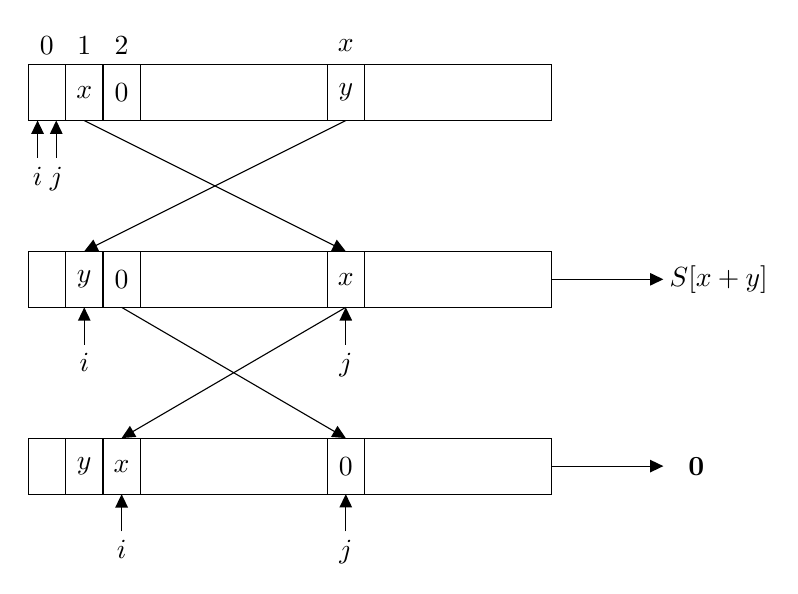
\begin{tikzpicture}[x=0.75pt,y=0.75pt,yscale=-0.9,xscale=0.9]
%uncomment if require: \path (0,303); %set diagram left start at 0, and has height of 303

%Shape: Rectangle [id:dp12455223677881988] 
\draw   (0,20) -- (280,20) -- (280,50) -- (0,50) -- cycle ;
%Straight Lines [id:da3353739678793939] 
\draw    (20,20) -- (20,50) ;
%Straight Lines [id:da058061035765641256] 
\draw    (40,20) -- (40,50) ;
%Straight Lines [id:da42003550403995904] 
\draw    (60,20) -- (60,50) ;
%Straight Lines [id:da10598677326132577] 
\draw    (160,20) -- (160,50) ;
%Straight Lines [id:da42710162603214696] 
\draw    (180,20) -- (180,50) ;
%Straight Lines [id:da7092047350089796] 
\draw    (5,69.98) -- (5,53) ;
\draw [shift={(5,50)}, rotate = 90] [fill={rgb, 255:red, 0; green, 0; blue, 0 }  ][line width=0.08]  [draw opacity=0] (7.14,-3.43) -- (0,0) -- (7.14,3.43) -- cycle    ;
%Straight Lines [id:da7389728658839063] 
\draw    (15,70) -- (15,53) ;
\draw [shift={(15,50)}, rotate = 90] [fill={rgb, 255:red, 0; green, 0; blue, 0 }  ][line width=0.08]  [draw opacity=0] (7.14,-3.43) -- (0,0) -- (7.14,3.43) -- cycle    ;
%Shape: Rectangle [id:dp33013142617767177] 
\draw   (0,120) -- (280,120) -- (280,150) -- (0,150) -- cycle ;
%Straight Lines [id:da7210338197084765] 
\draw    (20,120) -- (20,150) ;
%Straight Lines [id:da3654486767931029] 
\draw    (40,120) -- (40,150) ;
%Straight Lines [id:da785172840629027] 
\draw    (60,120) -- (60,150) ;
%Straight Lines [id:da902607613996435] 
\draw    (160,120) -- (160,150) ;
%Straight Lines [id:da5596828019899134] 
\draw    (180,120) -- (180,150) ;
%Straight Lines [id:da6056888258945672] 
\draw    (30,170) -- (30,153.02) ;
\draw [shift={(30,150.02)}, rotate = 90] [fill={rgb, 255:red, 0; green, 0; blue, 0 }  ][line width=0.08]  [draw opacity=0] (7.14,-3.43) -- (0,0) -- (7.14,3.43) -- cycle    ;
%Straight Lines [id:da7171343865291044] 
\draw    (170,170) -- (170,153) ;
\draw [shift={(170,150)}, rotate = 90] [fill={rgb, 255:red, 0; green, 0; blue, 0 }  ][line width=0.08]  [draw opacity=0] (7.14,-3.43) -- (0,0) -- (7.14,3.43) -- cycle    ;
%Shape: Rectangle [id:dp9326071824060944] 
\draw   (0,220) -- (280,220) -- (280,250) -- (0,250) -- cycle ;
%Straight Lines [id:da32531376385050326] 
\draw    (20,220) -- (20,250) ;
%Straight Lines [id:da6637069080324498] 
\draw    (40,220) -- (40,250) ;
%Straight Lines [id:da7451734861474262] 
\draw    (60,220) -- (60,250) ;
%Straight Lines [id:da34199443490066694] 
\draw    (160,220) -- (160,250) ;
%Straight Lines [id:da39996344557442587] 
\draw    (180,220) -- (180,250) ;
%Straight Lines [id:da9403812437728272] 
\draw    (50,270) -- (50,253.02) ;
\draw [shift={(50,250.02)}, rotate = 90] [fill={rgb, 255:red, 0; green, 0; blue, 0 }  ][line width=0.08]  [draw opacity=0] (7.14,-3.43) -- (0,0) -- (7.14,3.43) -- cycle    ;
%Straight Lines [id:da227200350400379] 
\draw    (170,270) -- (170,253) ;
\draw [shift={(170,250)}, rotate = 90] [fill={rgb, 255:red, 0; green, 0; blue, 0 }  ][line width=0.08]  [draw opacity=0] (7.14,-3.43) -- (0,0) -- (7.14,3.43) -- cycle    ;
%Straight Lines [id:da6637920376428952] 
\draw    (30,50) -- (167.32,118.66) ;
\draw [shift={(170,120)}, rotate = 206.57] [fill={rgb, 255:red, 0; green, 0; blue, 0 }  ][line width=0.08]  [draw opacity=0] (7.14,-3.43) -- (0,0) -- (7.14,3.43) -- cycle    ;
%Straight Lines [id:da09619501250612306] 
\draw    (170,50) -- (32.68,118.66) ;
\draw [shift={(30,120)}, rotate = 333.44] [fill={rgb, 255:red, 0; green, 0; blue, 0 }  ][line width=0.08]  [draw opacity=0] (7.14,-3.43) -- (0,0) -- (7.14,3.43) -- cycle    ;
%Straight Lines [id:da7693759914121461] 
\draw    (50,150) -- (167.41,218.49) ;
\draw [shift={(170,220)}, rotate = 210.26] [fill={rgb, 255:red, 0; green, 0; blue, 0 }  ][line width=0.08]  [draw opacity=0] (7.14,-3.43) -- (0,0) -- (7.14,3.43) -- cycle    ;
%Straight Lines [id:da016149633534485508] 
\draw    (170,150) -- (52.59,218.49) ;
\draw [shift={(50,220)}, rotate = 329.74] [fill={rgb, 255:red, 0; green, 0; blue, 0 }  ][line width=0.08]  [draw opacity=0] (7.14,-3.43) -- (0,0) -- (7.14,3.43) -- cycle    ;
%Straight Lines [id:da23602771826509095] 
\draw    (280,135) -- (337,135) ;
\draw [shift={(340,135)}, rotate = 180] [fill={rgb, 255:red, 0; green, 0; blue, 0 }  ][line width=0.08]  [draw opacity=0] (7.14,-3.43) -- (0,0) -- (7.14,3.43) -- cycle    ;
%Straight Lines [id:da15064968040726168] 
\draw    (280,235) -- (337,235) ;
\draw [shift={(340,235)}, rotate = 180] [fill={rgb, 255:red, 0; green, 0; blue, 0 }  ][line width=0.08]  [draw opacity=0] (7.14,-3.43) -- (0,0) -- (7.14,3.43) -- cycle    ;

% Text Node
\draw (10,10) node    {$0$};
% Text Node
\draw (30,10) node    {$1$};
% Text Node
\draw (50,10) node    {$2$};
% Text Node
\draw (170,10) node    {$x$};
% Text Node
\draw (30,35) node    {$x$};
% Text Node
\draw (50,35) node    {$0$};
% Text Node
\draw (170,35) node    {$y$};
% Text Node
\draw (5,73.38) node [anchor=north] [inner sep=0.75pt]    {$i$};
% Text Node
\draw (15,73.4) node [anchor=north] [inner sep=0.75pt]    {$j$};
% Text Node
\draw (30,135) node    {$y$};
% Text Node
\draw (50,135) node    {$0$};
% Text Node
\draw (170,135) node    {$x$};
% Text Node
\draw (30,173.4) node [anchor=north] [inner sep=0.75pt]    {$i$};
% Text Node
\draw (170,173.4) node [anchor=north] [inner sep=0.75pt]    {$j$};
% Text Node
\draw (30,235) node    {$y$};
% Text Node
\draw (50,235) node    {$x$};
% Text Node
\draw (170,235) node    {$0$};
% Text Node
\draw (50,273.4) node [anchor=north] [inner sep=0.75pt]    {$i$};
% Text Node
\draw (170,273.4) node [anchor=north] [inner sep=0.75pt]    {$j$};
% Text Node
\draw (342,135) node [anchor=west] [inner sep=0.75pt]    {$S[ x+y]$};
% Text Node
\draw (352,235) node [anchor=west] [inner sep=0.75pt]    {$\mathbf{0}$};


\end{tikzpicture}
	\caption{引理 \ref{lemma:3-8} 的证明}
	\label{fig:3-13}
\end{figure}

Mantin-Shamir 区分器表明,RC4 输出的第二字节是有偏差的。AlFardan 等人推广了这一结论,他们测量了许多随机密钥上的偏差,并表明,输出的前 $256$ 字节中的每一个都有偏差:每个字节的分布都与均匀性相去甚远 \cite{alfardan2013security}。这种偏差不像第二字节那样明显,但它仍是不可忽略不计的,并且足以用来对密码发动攻击。例如,他们表明,给定用 $2^{30}$ 个随机密钥加密的单一明文的对应密文,我们有可能以接近 $1$ 的概率恢复明文的前 $128$ 字节。这种攻击很容易在网络上进行,因为在网络上,一个秘密的 cookie 通常会被嵌入到一个消息的前几个字节中。每当浏览器连接到受害者的网络服务器时,这个 cookie 都会用新的密钥重新加密。攻击者可以使用 JavaScript 脚本令用户的浏览器反复重连到目标网站,以向攻击者提供发动攻击和暴露 cookie 所需的 $2^{30}$ 条密文。

作为回应,RSA 实验室发布了一项建议,建议放弃 RC4 流生成器输出的前 $1024$ 字节,而只使用第 $1025$ 字节及以后的字节。这可以防御最初的密钥流偏差区分器,但不能防御我们接下来将要讨论的攻击。

\begin{snote}[RC4 流生成器中的偏差。]
假设 RC4 设置算法已经被修改,从而使得上面介绍的攻击无效。Fluhrer 和 McGrew 给出了一个直接针对流生成器的攻击 \cite{fluhrer2000statistical}。他们声称字节对 $(0,0)$ 在 RC4 的输出中出现的次数多于它本应在随机序列中出现的次数。这足以将 RC4 的输出与随机序列区分开来。

令 $\mathrm{ST}_\mathrm{RC4}$ 为 RC4 所有可能的内部状态的集合。由于数组 $S$ 有 $n!$ 种可能的设置,而 $i$ 和 $j$ 各有 $n$ 种可能的设置,所以 $\mathrm{ST}_\mathrm{RC4}$ 的大小为 $n!\cdot n^2$。由于在 RC4 中 $n=256$,所以 $\mathrm{ST}_\mathrm{RC4}$ 的规模是非常巨大的,大约为 $10^{511}$。
\end{snote}

\begin{lemma}[Fluhrer-McGrew 定理]\label{lemma:3-9}
假设 RC4 由 $\mathrm{ST}_\mathrm{RC4}$ 中的一个随机状态 $T$ 初始化。令 $(z_1,z_2)$ 是 RC4 在状态 $T$ 下启动时输出的前两个字节。则有:
\[
\begin{aligned}
& i\neq n−1 & \Longrightarrow & \quad\Pr[(z_1,z_2)=(0,0)]\geq(1/n^2)\cdot\big(1+(1/n)\big)\\
& i\neq 0,1 & \Longrightarrow & \quad\Pr[(z_1,z_2)=(0,1)]\geq(1/n^2)\cdot\big(1+(1/n)\big)
\end{aligned}
\]
\end{lemma}

我们将一对连续输出 $(z_1,z_2)$ 称为一个\textbf{二重字(digraph)}。在一个真随机序列中,所有的二重字 $(x,y)$ 出现的概率都应当正好是 $1/n^2$。但上面的引理表明,对于 RC4,$(0,0)$ 出现的概率比它应有的值大 $1/n^3$。$(0,1)$ 也是如此。事实上,除了引理 \ref{lemma:3-9} 所述的两个二重字,Fluhrer-McGrew 还确定了其他几个异常的二重字。

该引理导出了一个简单的区分 RC4 输出和随机序列的区分器 $D$。如果区分器在给定的序列中发现的 $(0,0)$ 的数量大于随机序列中应有的数量,它就输出 $1$,否则就输出 $0$。

\vspace*{10pt}

\hspace*{5pt} 输入:序列$s\in\{0,\dots,n\}^\ell$\\
\hspace*{26pt} 输出:$0$ 或 $1$

\vspace{5pt}

\hspace*{5pt} 令 $q$ 为 $x$ 中出现二重字 $(0,0)$ 的次数\\
\hspace*{26pt} 如果 $(q/\ell)-(1/n^2)>1/(2n^3)$ 则输出 $0$,否则输出 $1$

\vspace*{10pt}

使用定理 \ref{theo:B-3},我们可以估计出 $D$ 的优势与输入长度 $\ell$ 的关系。特别地,区分器 $D$ 能获得下述优势:
\[
\begin{aligned}
\ell=2^{14}\text{ 字节}: &\quad\quad \mathrm{PRG}\mathsf{adv}[D,RC4]\geq2^{-8}\\
\ell=2^{34}\text{ 字节}: &\quad\quad \mathrm{PRG}\mathsf{adv}[D,RC4]\geq0.5
\end{aligned}
\]
使用 Fluhrer 和 McGrew 提供的所有异常二重字,我们就可以建立一个区分器,只用 $2^{30.6}$ 字节的输出,就能实现 $0.8$ 的优势。

\begin{snote}[针对 RC4 的相关密钥攻击。]
Fluhrer、Mantin 和 Shamir 表明,RC4 与相关密钥一起使用时是不安全的 \cite{fluhrer2001weaknesses}。我们将在 \ref{sec:9-10} 节的攻击 $2$ 中讨论这种攻击及其对 802.11b WiFi 协议的影响。
\end{snote}